% =========================================================================
% Appendix E — sub-axes (hover / grav / cloak / teleport / sim). FILLED.
%   folds UFO/{grav,cloak,hexa-teleport,hexa-sim,hexa-hover}/*.md:
%   per-axis spec fold (HEXA-HOVER/GRAV/CLOAK/TELEPORT/SIM), the teleport
%   superluminal WHITE fence, the falsifier-count summary, and a pgfplots
%   sub-axis falsifier-count chart. Honest: these orbit the ladder; the
%   speculative parts stay WHITE-fenced.
% =========================================================================
\section{Sub-Axes --- Hover, Grav, Cloak, Teleport, Sim}
\label{app:subaxes}

This appendix folds the five UFO sub-axes that surround the propulsion
ladder. \textbf{HEXA-HOVER} is the Meissner-levitation canon
(RTSC \SI{48}{\tesla} solenoid cross-link, HTS REBCO primary conductor,
Earnshaw \citep{earnshaw1842} active feedback). \textbf{HEXA-GRAV} is a
gravity-sensing axis (LIGO-miniature gravitational-wave arm
$h\!\sim\!10^{-23}$, atom-interferometer $\Delta g\!\sim\!10^{-11}g$ with
SQUID readout, RTSC $\mu$-metal $\times5$ EM/inertial separation, four
preregistered falsifiers). \textbf{HEXA-CLOAK} is an EM-visibility shell
(transformation-optics $\varepsilon$-$\mu$ tensor metamaterial,
RCS $10^{-6}$\,m$^2$ $+$ IR reduction, the stage-propulsion-EM-leak vs.\
cloak compatibility budget, four falsifiers). \textbf{HEXA-TELEPORT} is
the standard quantum-teleportation protocol (Bell-pair $+$ Bell-state
measurement $+$ classical channel $\le c$ $+$ unitary, entanglement
swapping relay, with the superluminal-communication / no-cloning claim
\tierWhite\ \textsc{Speculation-Fenced}, and a QKD BB84/E91 application).
\textbf{HEXA-SIM} is the digital-twin simulation engine (integrated CFD
$+$ EM $+$ propulsion) that drives the verb-4 \texttt{analyze}\,$\circlearrowleft$.

% -------------------------------------------------------------------------
\subsection{The five sub-axis fold}
\label{app:subaxes-table}

Table~\ref{tab:subaxes} is the per-axis summary: the physical mechanism,
the headline number (transcribed from the source spec, not invented), the
ladder coupling, and the honest tier of the load-bearing claim.

\begin{table}[h]
\centering
\small
\setlength{\tabcolsep}{4pt}
\begin{tabular}{@{}l >{\raggedright\arraybackslash}m{3.0cm} >{\raggedright\arraybackslash}m{3.0cm} >{\raggedright\arraybackslash}m{2.4cm} c@{}}
\toprule
\textbf{axis} & \textbf{mechanism} & \textbf{headline number} & \textbf{ladder coupling} & \textbf{tier} \\
\midrule
HEXA-HOVER & Meissner $\chi_v{=}-1$ levitation & $F_{\text{lev}}{\sim}1.59{\times}10^6$\,N (App.~\ref{app:stage1}) & Stage-1 (RTSC) & \tierGreen \\
HEXA-GRAV & SC interferometer + atom-IF + SQUID & $h{\sim}10^{-23}$, $\Delta g{\sim}10^{-11}g$ & nav/sensing & \tierYellow \\
HEXA-CLOAK & transformation-optics $\varepsilon$-$\mu$ metamaterial & RCS ${\sim}10^{-6}$\,m$^2$ & EM-leak budget & \tierYellow \\
HEXA-TELEPORT & Bell-pair + BSM + classical ch.\ $\le c$ & QKD BB84/E91 link & comms (off-ladder) & \tierGreen/\tierWhite \\
HEXA-SIM & integrated CFD+EM+propulsion twin & 4-layer $\circlearrowleft$ solver & verb-4 engine & \tierOrange \\
\bottomrule
\end{tabular}
\caption{The five UFO sub-axes
(\texttt{UFO/\{hover,grav,cloak,hexa-teleport,hexa-sim\}/*.md}). Headline
numbers are transcribed from each source spec, not recomputed here. Only
HEXA-HOVER carries a \tierGreen\ closed-form atom (the Stage-1 lift,
App.~\ref{app:stage1}); HEXA-GRAV and HEXA-CLOAK are
\tierYellow\ \textsc{Supported-By-Citation} composite formulas;
HEXA-TELEPORT is \tierGreen\ for the standard protocol but its
\emph{superluminal} interpretation is \tierWhite\ fenced; HEXA-SIM is the
\tierOrange\ digital-twin engine (its heavy body-solves are the deferred
verb-4 gates, App.~\ref{app:gateinv}).}
\label{tab:subaxes}
\end{table}

% -------------------------------------------------------------------------
\subsection{The teleport superluminal fence}
\label{app:subaxes-teleport}

HEXA-TELEPORT is the one sub-axis with a built-in honesty fence. The
standard quantum-teleportation protocol (Bell pair, Bell-state
measurement, classical correction channel, unitary recovery) is
\tierGreen\ textbook physics and yields a real QKD (BB84/E91) link. But
teleportation transfers \emph{no information faster than the classical
channel}, which is bounded by $c$; the no-cloning theorem forbids copying
the state. Any reading of HEXA-TELEPORT as a \emph{superluminal
communication} channel is therefore \tierWhite\
\textsc{Speculation-Fenced} and explicitly UNPROVEN --- it sits on the
same epistemic shelf as the Stage-4--7 falsifiers, not on the Stage-1--3
proven ladder. The capstone keeps the protocol (proven) and the
superluminal claim (fenced) sharply separated, mirroring the
proven/UNPROVEN wall ($\wall$).

% -------------------------------------------------------------------------
\subsection{Sub-axis falsifier inventory}
\label{app:subaxes-falsifiers}

Each speculative sub-axis carries its own small preregister.
Fig.~\ref{fig:subaxes-fal} compares the falsifier counts: HEXA-GRAV
(EM/inertial separation, GW-band reach) and HEXA-CLOAK (EM-leak vs.\
cloak budget, broadband RCS) carry four each; HEXA-TELEPORT carries the
single superluminal fence; HEXA-HOVER and HEXA-SIM carry none of their
own (HEXA-HOVER's claim is the \tierGreen\ Stage-1 atom, HEXA-SIM's risk
is the deferred verb-4 body-solve, not a speculative proposition).

\begin{figure}[h]
\centering
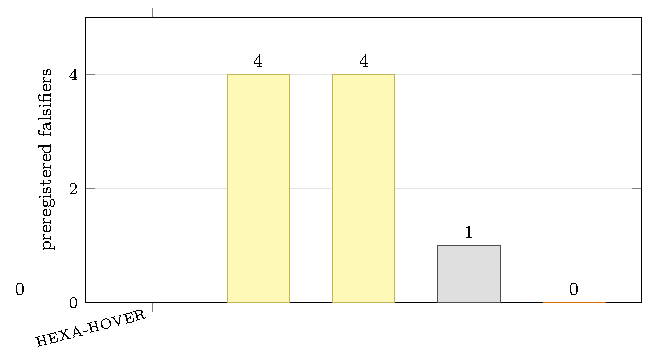
\includegraphics[width=0.80\linewidth]{figures/fig07_subaxis_falsifiers.pdf}
\caption{Preregistered falsifier counts per UFO sub-axis. HEXA-GRAV and
HEXA-CLOAK carry 4 each (speculative composite claims with named
measurands); HEXA-TELEPORT carries 1 (the superluminal fence). HEXA-HOVER
(\tierGreen\ closed-form lift) and HEXA-SIM (\tierOrange\ deferred
body-solve) carry none --- their honesty is enforced by tier, not by a
falsifier. The bar heights mirror how much of each sub-axis is
speculative vs.\ proven/deferred.}
\label{fig:subaxes-fal}
\end{figure}

% -------------------------------------------------------------------------
\subsection{Honest scope}
\label{app:subaxes-scope}

The sub-axes orbit the propulsion ladder; they are not new physics atoms.
HEXA-HOVER reuses the Stage-1 \tierGreen\ atom; HEXA-SIM \emph{is} the
verb-4 engine whose heavy solves are deferred (\tierOrange). HEXA-GRAV
and HEXA-CLOAK are \tierYellow\ cited composites with their own open
falsifiers, and HEXA-TELEPORT's superluminal reading is \tierWhite\
fenced. None of them moves the capstone's \texttt{absorbed=false}
verdict toward \texttt{true}, and none upgrades a speculative claim by
proximity to the proven ladder.
